\documentclass{scrartcl}
\usepackage{lscape}
\usepackage{tikz}

\begin{document}
\begin{landscape}
\centering
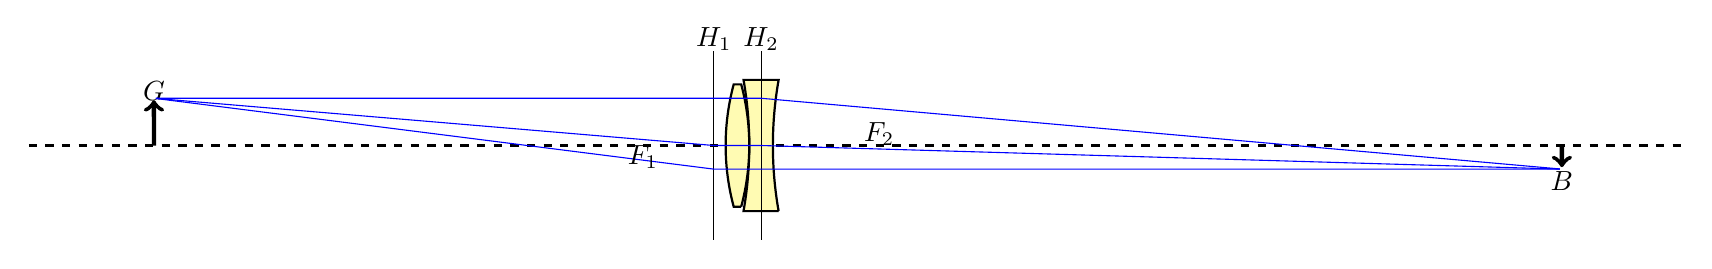
\begin{tikzpicture}[scale=0.3, inner sep=0]

% Optische Achse
\draw[dashed, thick] (-30,0) -- (40,0);
% Koordinaten Nullpunkt
\draw (0,-0.2) -- (0,0.2);

% Konkave Linse
\def\xconv{1} % x-Koordinate
\draw[thick, fill=yellow!30] 
     ([shift=(190:16cm)]16.5+\xconv,0) arc (190:170:16cm)
     -- ([shift=(10:16cm)] -16.5+\xconv,0)
     arc (10:-10:16cm) 
     -- ([shift=(190:16cm)]16.5+\xconv,0);

% Konvexe Linse
\def\xconx{-1} % x-Koordinate
\draw[thick, fill=yellow!30] ([shift=(-15:10cm)]-8.5+\xconx,0) arc (-15:15:10cm)
 --([shift=(165:10cm)]10.5+\xconx,0) arc (165:195:10cm)
 --([shift=(-15:10cm)]-8.5+\xconx,0);

% Gegenstand (Pfeil)
\def\Gx{-24.7}
\node (G) at (\Gx,2) {};
\draw[->, ultra thick] (\Gx,0) -- (G);%
\node (labG) at (\Gx,2.3) {$G$};
% Bild (arrow)
\def\Bx{34.9}
\node (B) at (\Bx,-1) {};
\draw[->, ultra thick] (\Bx,0) -- (B);
\node (labB) at (\Bx,-1.5) {$B$};

% Hauptebenen
\def\Hx{1}
\draw (\Hx,-4) -- (\Hx,4); % H1
\node (labH1) at (-\Hx,4.5) {$H_1$};
\draw (-\Hx,-4) -- (-\Hx,4); % H2
\node (labH2) at (\Hx,4.5) {$H_2$};

% Strahlen
% FokusG
\draw[color=blue] (G) -- (-\Hx,-1);
\draw[color=blue] (G) -- (\Hx,2);
% FokusB
\draw[color=blue] (B) -- (-\Hx,-1);
\draw[color=blue] (B) -- (\Hx,2);
%Central
\draw[color=blue] (G) -- (-\Hx,0) -- (\Hx,0)  -- (B);
               
% Label
%Fokus Punkte
\node (F1) at (-4,-0.5) {$F_1$};
\node (F2) at (6,0.5) {$F_2$};

% Gebogener Pfeil
%\draw[->, dashed] (9.5,18) .. controls (4,18) .. (3,11.65);
\end{tikzpicture}
\end{landscape}
\end{document}